\chapter{The \AC\ Approach}
\label{chap:argoncube}

To mitigate the drawbacks mentioned in Section~\ref{sec:lartpc_challenges}, the Bern group has founded the \AC\ collaboration, with the goal of developing a new fully-modular type of \lartpc.
Modularity reduces pile-up and allows for shorter drift-times, thus slackens the requirements on argon purity and HV.
A modular detector also contains light within each module, allowing for a more accurate trigger system.
Maintenance and upgrading of a modular detector is much easier than for a monolothic one.


\section{Modularity}
\label{sec:ac_modularity}

\AC\ is made of fully autarkic TPC modules.
In case of a fault condition the affected module(s) can be shut down and repaired or replaced individually without affecting the rest of the detector.
During construction, one can start data taking as soon as the first module is operational and needs not wait for the commissioning of the whole detector.
A modular detector furthermore reduces event pile-up because the acquisition time is reduced to the size of one module.
This is crucial in the high-multiplicity environments of future liquid argon neutrino detectors.
Finally, also trigger purity profits from a modular approach because scintillation light is contained within one module allowing for a localised trigger.

\begin{figure}[htb] %TODO: better, more recent picture
	\centering
	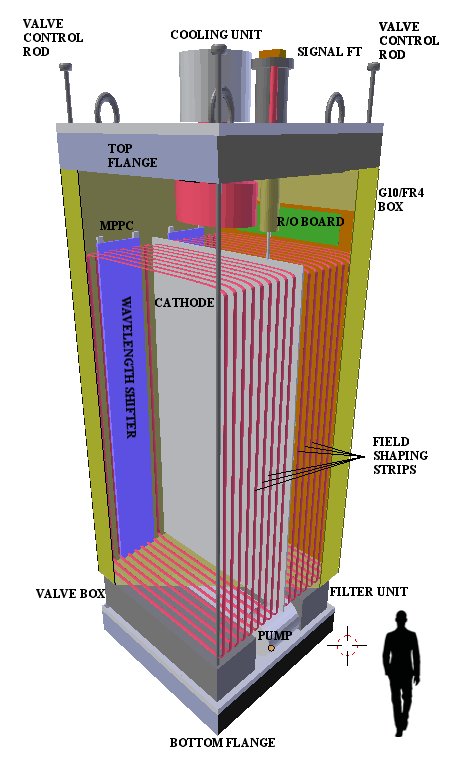
\includegraphics[height=.5\textheight]{ac/module}
	\caption{Schematic of an \AC\ module}
	\label{fig:ac_module}
\end{figure}

A module is made of a rectangular box with a square footprint and the height required by the detector design.
The top and bottom sides of the box are made from stainless steel while the sidewalls are made from FR-4.
FR-4 is a glass-reinforced epoxy composite widely used for printed circuit boards (PCBs).
The modules are placed side-by-side in a bath of liquid argon where they can be extracted and reinserted when needed.
Purity of the liquid argon is maintained within each module using an integrated recirculation system in the bottom of the module (see Section~\ref{sec:ac_cryo}).
As a result, the bath surrounding the modules needs not meet as stringent purity requirements as the argon inside.
Under normal operation conditions, all modules are inserted and the gaps between them are sealed off by indium seals pressed onto the top flanges.
The schematic of an \AC\ module is shown in Figure~\ref{fig:ac_module}.

To extract a module, the indium seal around the flange in question is removed and a drain pipe on the bottom of the module is opened.
The module is then slowly lifted up by a crane and the liquid argon is drained to the surrounding bath by means of gravity.
On the bottom of the module, a blind flange is located with equal dimensions as the top flange but without any feedthroughs.
When the bottom flange reaches the position of the top flange, it is sealed with indium again and then detached from the module which is now free and can be brought to its destination.
Upon reinsertion, the procedure is basically reversed.
First, the module is reattached to the blind flange and the indium seals is removed.
Then, the inner volume is opened to the surrounding bath to push the liquid argon into the module.
As opposed to extraction, the argon is guided through an oxygen trap as a first purification step.
The required pressure is supplied by the weight of the module floating on the liquid argon bath.
As soon as the top flange of the module reaches the top flanges of the other modules, the indium seal is reinstalled.
Figure~\ref{fig:ac_module-ins-ext} shows the insertion (left) and extraction (right) of a module.

\begin{figure}[htb] %TODO: better, more recent pictures?
	\centering
	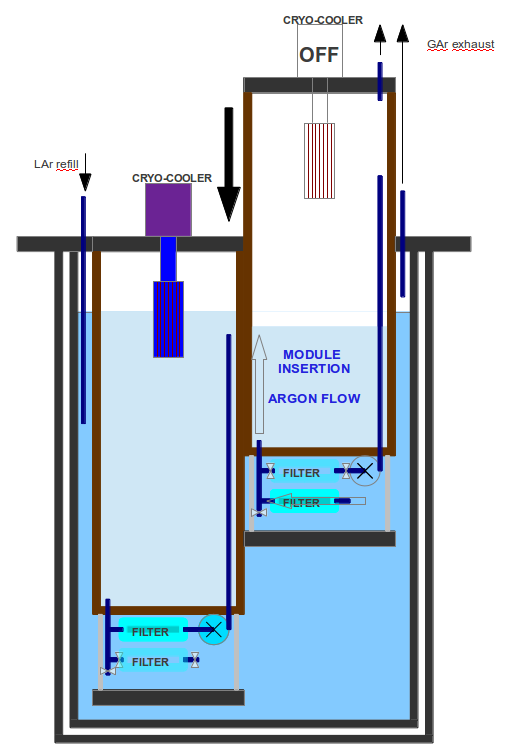
\includegraphics[width=.49\textwidth]{ac/module_insertion}
	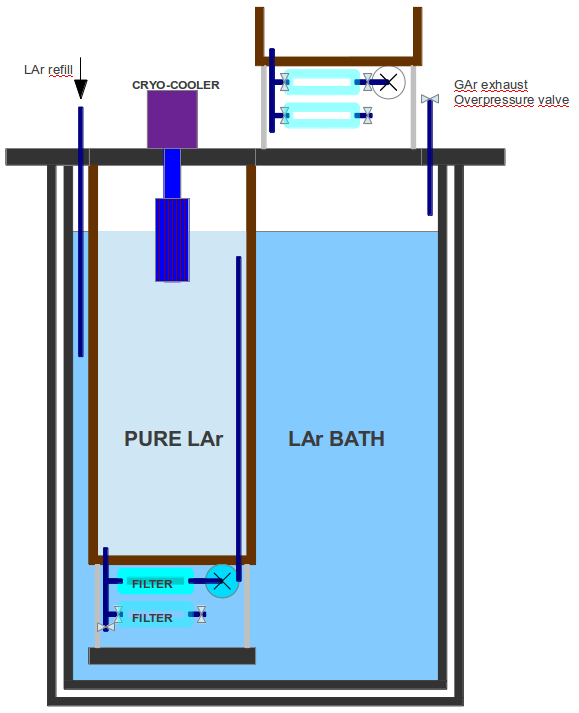
\includegraphics[width=.49\textwidth]{ac/module_extraction}
	\caption{Insertion (left) and extraction (right) of a module}
	\label{fig:ac_module-ins-ext}
\end{figure}

Another big problem that can be solved by a modular detector design are the high electric fields required for large detectors.
Because each module contains its own TPC independent of all other modules, the required cathode potential only depends on the module size not the detector size.
To minimise the cathode voltage, the field is applied along one of the short edges of a module and furthermore, the module is split in half by the cathode reducing the voltage by anoter factor of two.
Thus, for a module footprint of \SI{2 x 2}{\metre} and an electric field of \SI{1}{\kilo\volt\per\centi\metre}, a cathode potential of \SI{100}{\kilo\volt} is required.
Operating a \lartpc at this voltage is challenging but feasible without a prohibitive loss in fiducial volume~\cite{AT}.


\section{Cryogenics}
\label{sec:ac_cryo}


\section{Charge Readout}
\label{sec:ac_charge-readout}


\section{Light Readout}
\label{sec:ac_light-readout}